\newpage
\section{Memory Hierarchy Design Basics}
\begin{figure}[!htb]
    \centering
    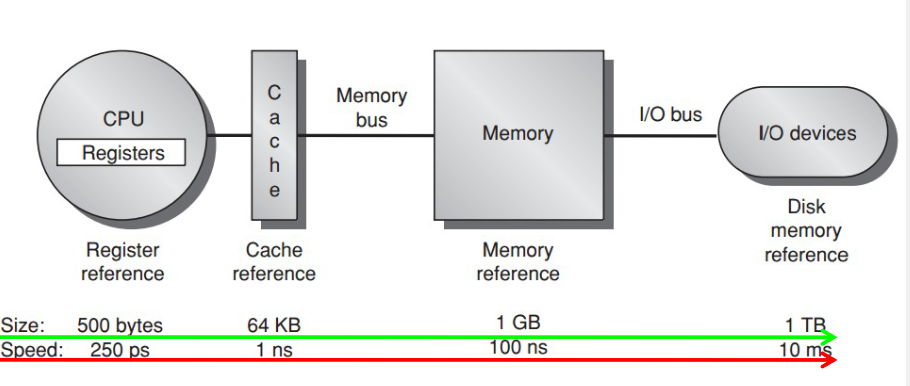
\includegraphics[width=0.309\textwidth]{pic/CA2/Memory Hierarchy}
    \caption{Memory Hierarchy}
\end{figure}

\subsection{Technology \& Optimizations}
\begin{figure}[!htb]
    \centering
    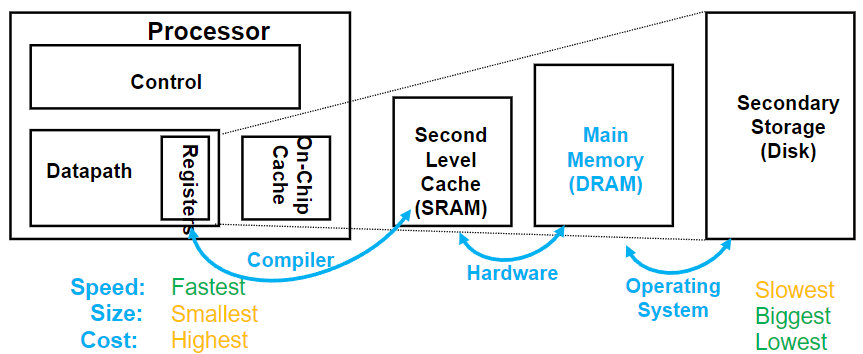
\includegraphics[width=0.309\textwidth]{pic/CA2/Main Memory}
    \caption{Main Memory}
\end{figure}

Performance measures
\begin{itemize}
    \item Latency: the time to retrieve the first word of the block
    \begin{itemize}
        \item access time: 从请求到数据到达的时间
        \item cycle time: 从一个 access 开始到另一个 access 开始相距的时间
    \end{itemize}
    \item Bandwidth: the time to retrieve the rest of this block
\end{itemize}

\subsubsection{SRAM for cache}
Static Random Access Memory(SRAM)

\begin{itemize}
    \item Direct Mapped Cache %TODO 15
    \item Set Associative Cache 
    \item Fully Associative Cache
\end{itemize}
信息 bit 为需要根据具体情况确定. 

e.g 16KB direct mapped cache 256byte blocks. Assume 1words=8bits\\
use $\log_2256=8$-bit offset, $16kB/256B=64$ lines, $\log_2(64)=6$-bit line index. 

\subsubsection{DRAM for main memory}
\begin{itemize}
    \item Dynamic Random Access Memory(DRAM)
    \item Single transistor per bit
    \item Reading destroys the information
    \item Refresh periodically
    \item cycle time > access time
\end{itemize}

\begin{figure}[!htb]
    \centering
    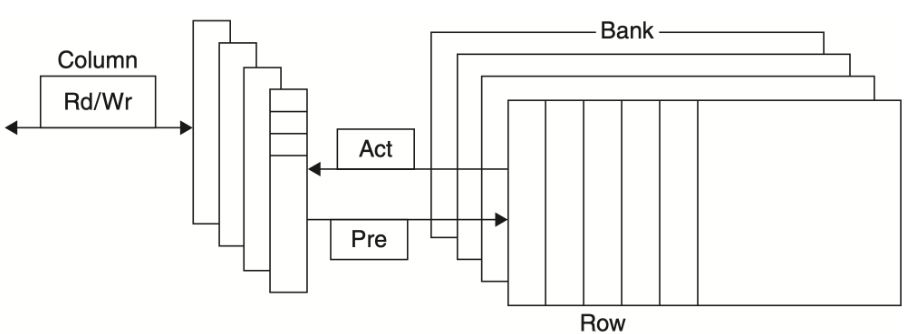
\includegraphics[width=0.309\textwidth]{pic/CA2/DRAM Organization}
    \caption{DRAM Organization}
\end{figure}

DRAM Access Example

\subsubsection{DRAM Improvement}
\begin{itemize}
    \item Timing signals
    \item Leverage spatial locality
    \item Clock signal
    \item SDRAM
    \item Wider DRAM
    \item DDR: double data rate
    \item Multiple Banks
    \item Reducing power consumption in SDRAMs
\end{itemize}

\subsection{Cache Performance}
Average Memory Access Time = Hit Time + Miss Rate x Miss Penalty

Six Basic Cache Optimizations:
\begin{enumerate}\small
    \item larger block size
    \item bigger caches
    \item higher associativity
    \item multilevel caches
    \item giving priority to read misses over writes
    \item avoiding address translation during indexing of the cache
\end{enumerate}

Root Causes of Miss Rates:
\begin{itemize}
    \item Compulsory: $\overset{\text{冷启动/首次未命中}}{\text{cold-start/first-reference misses}}$
    \item Capacity: cache size limit
    \subitem occur upon the cache is full
    \item Conflict: collision misses
    \subitem occur without the cache being fully occupied
\end{itemize}

\subsubsection{Larger Block Size}
\begin{itemize}
    \item Reduce compulsory misses
    \subitem Leverage spatial locality
    \item Increase conflict/capacity misses
    \subitem Fewer blocks in the cache
    \subitem Larger blocks increase miss penalty
\end{itemize}

\subsubsection{Larger Cache}
\begin{itemize}
    \item Reduce capacity misses
    \item Increase hit time, cost, and power
\end{itemize}

\subsubsection{Higher Associativity}
\begin{itemize}
    \item Reduce conflict misses
    \item Increase hit time
\end{itemize}

2:1 cache rule of thumb: a direct-mapped cache of size $N$ has about the same miss rate as a two-way set associative cache of size $N/2$

\subsubsection{Multilevel Cache}
Reduce miss penalty

\begin{figure}[!htb]
    \centering
    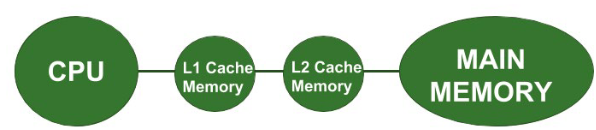
\includegraphics[width=0.309\textwidth]{pic/CA2/Multilevel Cache}
    \caption{Multilevel Cache}
\end{figure}

Two-level cache: Add another level of cache between the original cache and memory.
\begin{itemize}
    \item L1: small enough 来匹配处理器的 clock time
    \item L2: large enough 来存储要去主存的访问, 减少 miss penalty
\end{itemize}

Local miss rate and Global miss rate

Multilevel inclusion and Multilevel exclusion

\subsubsection{Prioritize Read Misses Over Writes}
Reduce miss penalty

读写操作分开对待. check the contents of write buffer, let the read miss continue if no conflicts with write buffer \& memory system is available


\subsubsection{Avoid Address Translation During Indexing Cache}
Cache addressing
\begin{itemize}
    \item virtual address -- virtual cache
    \item physical address -- physical cache
\end{itemize}
Processor/program -- virtual address

Processor $\to$ address translation $\to$ Cache

Virtually indexed(TLB), physically tagged

并行执行虚拟地址的转换与地址查找, 提高缓存命中的时间. 


e.g. %TODO P141-150 and 152 两个例子, 图 + 信息

% textbook Chapter 2.1-2.2 Appendix B

\newpage
\section{Memory Hierarchy Design Advances}
\subsection{Ten Advanced Cache Optimizations}
Goal: average memory access time down. 

Metrics to reduce/optimize:
\begin{itemize}
    \item hit time
    \item miss rate
    \item miss penalty
    \item cache bandwidth
    \item power consumption
\end{itemize}

\subsubsection{Small and Simple First-Level Caches}
Small size: support a fast clock cycle and reduce power

Lower associativity: reduce both hit tme and power

\subsubsection{Way Prediction}
Reduce conflict misses and hit time. 

block predictor bits are added to each block to predict the way/block within the set of the next cache access. Used in a cache with more than one
block in a set. 

\subsubsection{Pipelined Access and Multibanked Caches}
Increase cache bandwidth. with Higher latency and Greater penalty. 

Divide cache into independent banks that support simultaneous accesses.

Sequential interleaving  spread the addresses of blocks sequentially across the banks. 
 
\begin{figure}[!htb]
    \centering
    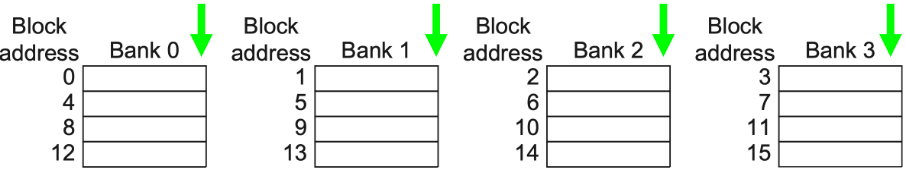
\includegraphics[width=0.42\textwidth]{pic/CA2/Multibanked Caches}
    \caption{Multibanked Caches}
\end{figure}

\subsubsection{Nonblocking Caches}
Increase cache bandwidth. 

Nonblocking/lockup-free cache leverage out-of-order execution, allows data cache to continue to supply cache hits during a miss. 

\subsubsection{Critical Word First and Early Restart}
Reduce miss penalty. Motivation: processor normally needs just one word of the block at a time. 

Critical word first: request the missed word first from the memory and send it to the processor as soon as it arrives;

Early restart: fetch the words in normal order, as soon as the requested word arrives send it to the processor

\subsubsection{Merging Write Buffer}
Reduce miss penalty

Write merging merges four entries (with sequential addresses) into a single buffer entry

\subsubsection{Compiler Optimization}
Reduce miss rates, w/o hw changes

\begin{enumerate}
    \item [Tech 1] Loop interchange: exchange the nesting of the loops to make the code access the data in the order in which they are stored
    \item [Tech 2] Blocking: compute using submatrices after; maximize accesses to loaded data before they are replaced
\end{enumerate}

\subsubsection{Hardware Prefetching}
Reduce miss penalty/rate

Prefetch items before the processor requests them, into the cache or external buffer

Instruction prefetch

\subsubsection{Compiler Prefetching}
Reduce miss penalty/rate

Compiler to insert prefetch instructions to request data before the processor needs it

\begin{itemize}
    \item Register prefetch
    \item Cache prefetch
\end{itemize}%TODO 看例子, 有点没理解

\subsubsection{HBM}
Use HBM as L4 cache(垂直空间)

\subsection{Virtual Memory and Virtual Machine}
考试不考, 摸了. % 自己看书看 ppt, 